\chapter{An Overview of Temporal, Sensitivity and Uncertainty Analyses}\label{ch:background}
%\setlength{\epigraphwidth}{0.75\textwidth}
%\epigraph{\textit{A product should be designed in such a way that makes its performance insensitive to variation in variables beyond the control of the designer.}}{\textit{Genichi Taguchi}}

In this chapter, we review implicit time marching methods for flexible multibody dynamics as well as methods for sensitivity analysis and uncertainty quantification.
Finally, the specific objectives of the thesis are discussed.

\section{Temporal Analysis of Physics: Flexible Multibody Dynamics}
\begin{figure}[h!]
  \centering
  \begin{subfigure}{0.49\textwidth}
    \centering
    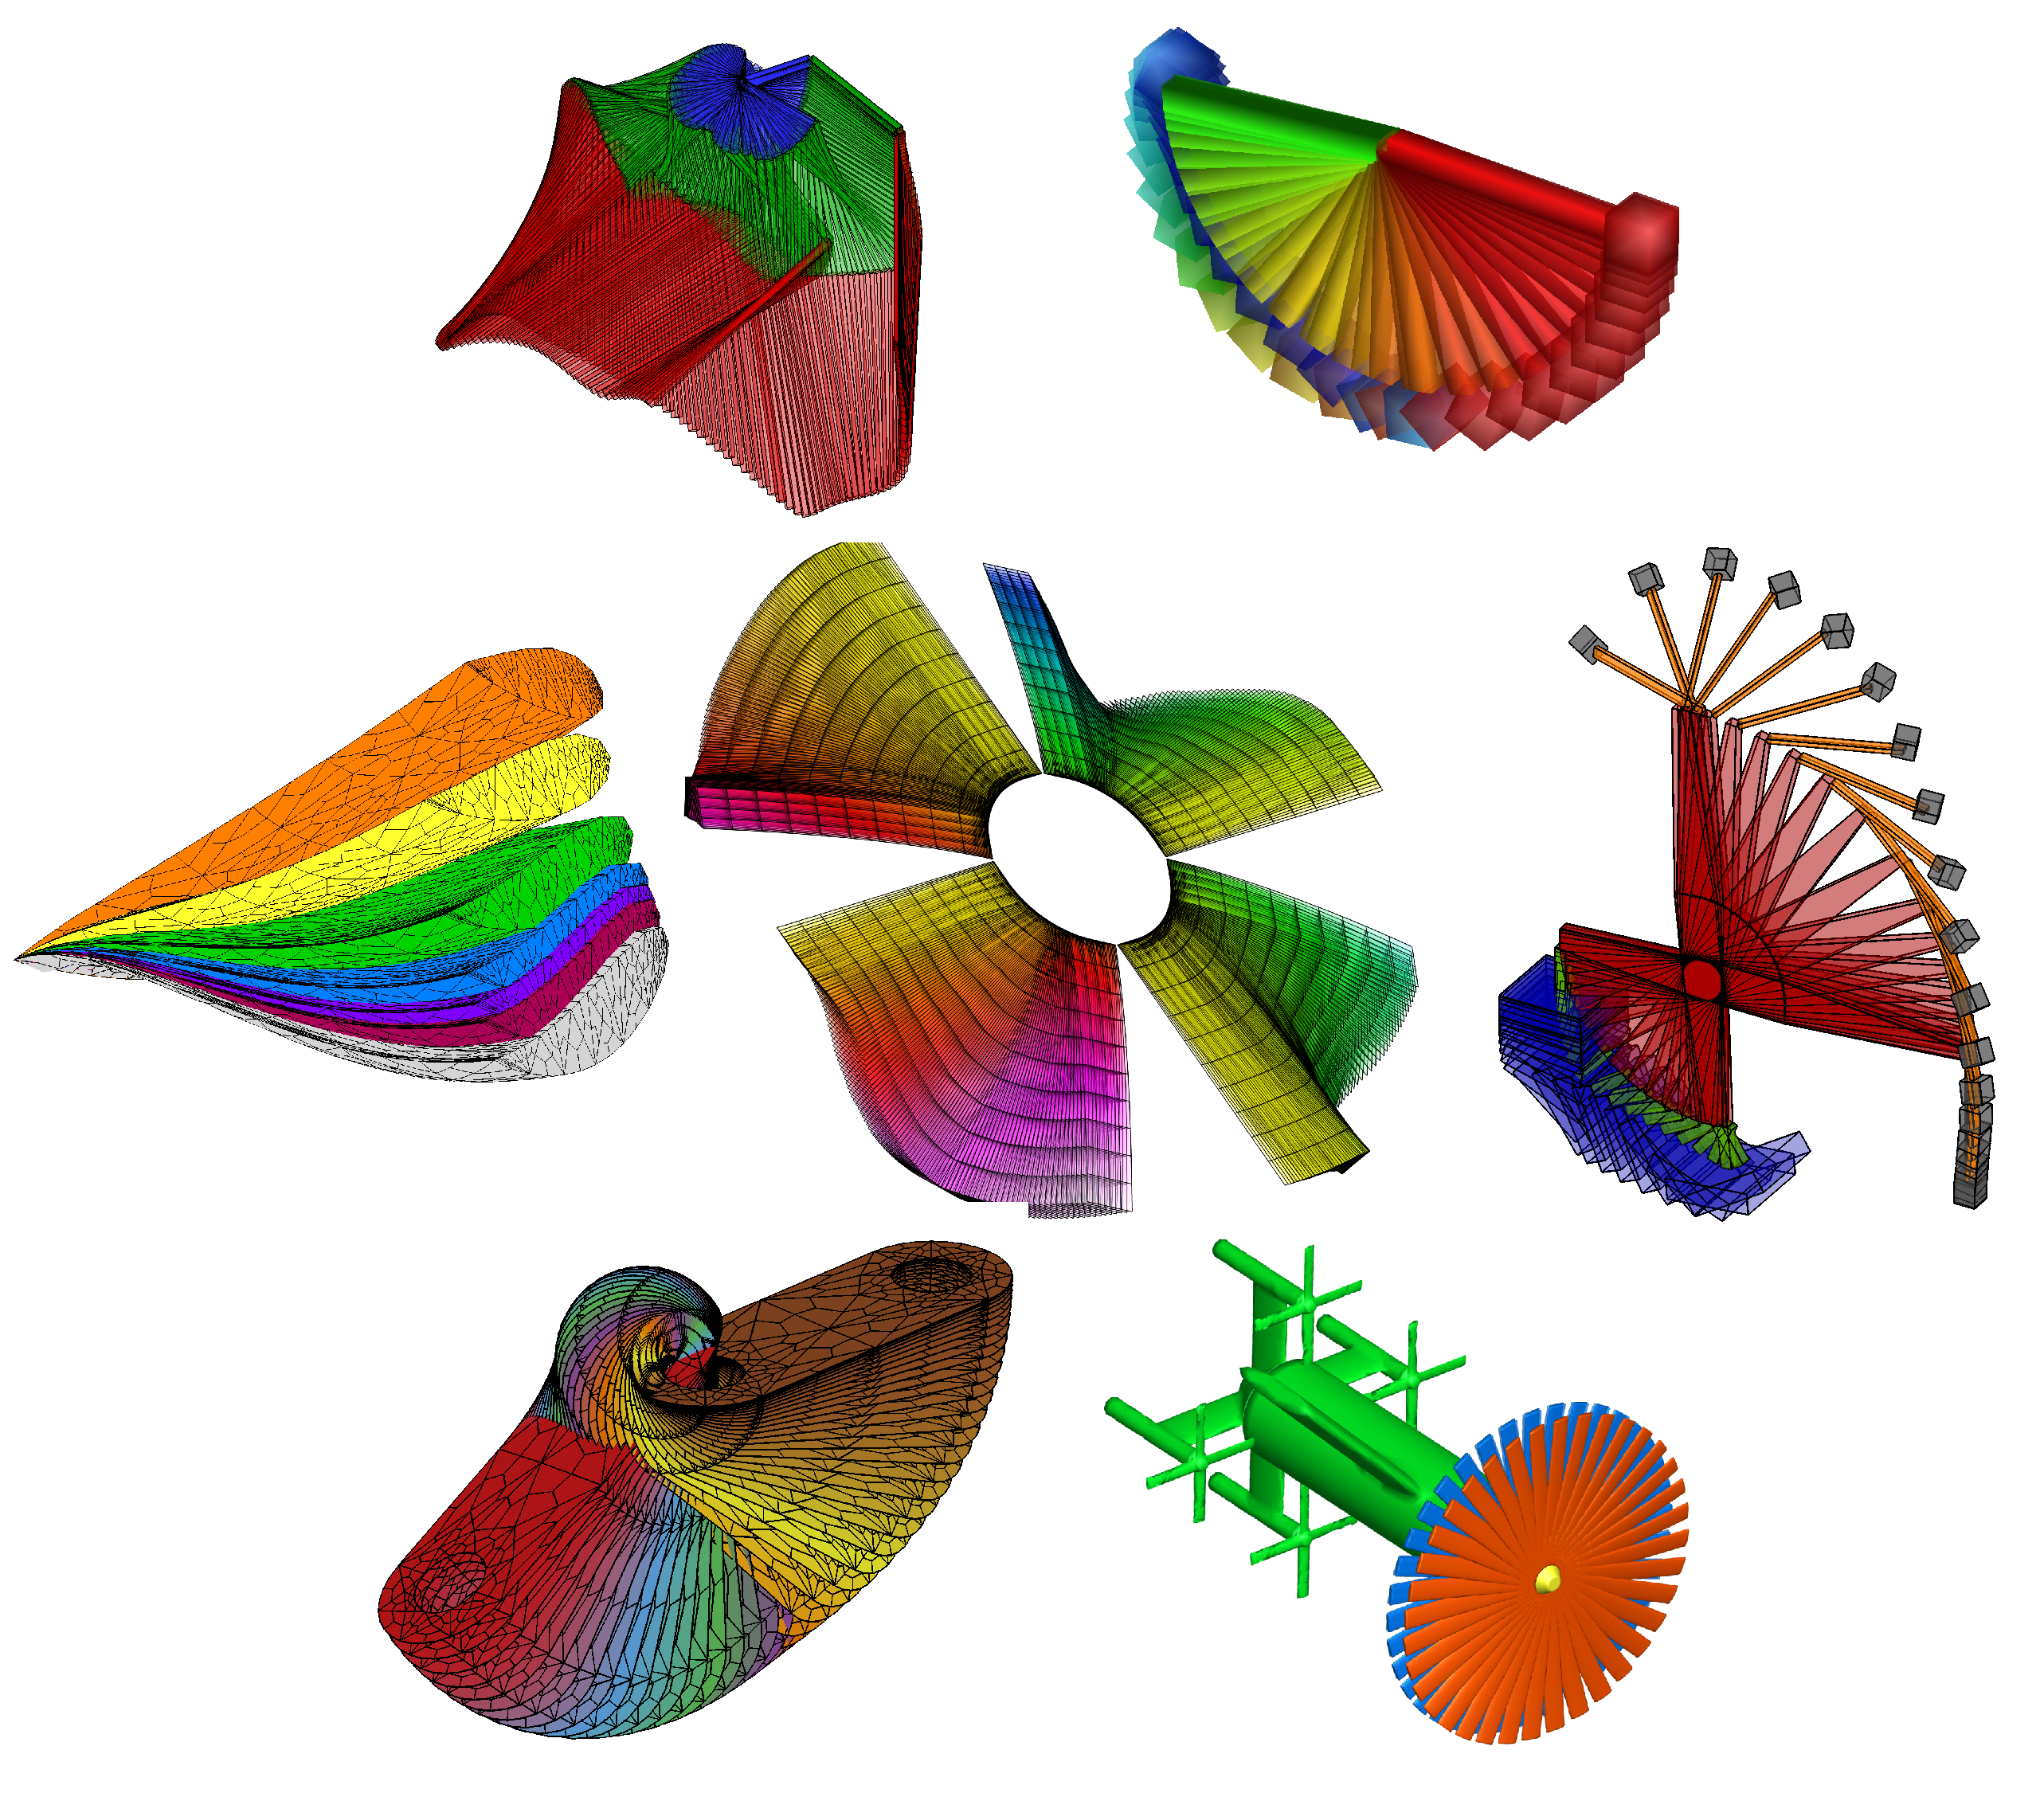
\includegraphics[trim=1pt 1pt 1pt 1pt,clip,width=\linewidth]{mbdyn.pdf}
  \end{subfigure}
  \begin{subfigure}{0.49\textwidth}
    \centering
    \includegraphics[trim=1pt 1pt 1pt 1pt,clip,width=\linewidth]{helix.png}
  \end{subfigure}
  \caption{Timelapse and timespirals depicting temporal evolution of dynamical
    systems.}
  \label{fig:time-lapse-spiral-example}
\end{figure}
\subsection{Abstract Form of Governing Equations}
The temporal evolution of some flexible multibody systems are shown in Figure~\ref{fig:time-lapse-spiral-example}.
Such systems can be studied by solving a system of nonlinear ordinary differential/algebraic equations of the form:
\begin{equation}\label{eqn:abstract-residual-form}
  R(t, \xi, u(t,\xi), \dot{u}(t,\xi), \ddot{u}(t,\xi)) = 0,
\end{equation}
where $u(t,\xi)$ is a function that describes the physical state of the system, along with functions describing the time rate of change: $\dot{u}(t,\xi)$ and $\ddot{u}(t,\xi)$. Here $t$ is the temporal variable and $\xi$ is the design variable.
In principle, the abstract descriptor form~\eqref{eqn:abstract-residual-form} form facilitates the treatment of different formulations and discretizations of the governing equations, as well as governing equations for different physics under a common mathematical framework.
For example, Equation~\eqref{eqn:abstract-residual-form} can be viewed as an abstract representation of time dependent processes resulting from:
\begin{itemize}
\item purely algebraic equations (e.g. spring mass damper system, Van der Pol oscillator) or
\item algebraic equations resulting from spatial discretization (e.g. beam deformation model, Laplace equation) or
\item algebraic equations of a particular physics resulting from different formulations (e.g. Newton--Euler method, Maggi's method, Euler--Lagrange method, Hamilton's principle~\cite{Bachau:Flexible-multibody-dynamics,Meirovitch1997}).
\end{itemize}
%The state function $u(t)$ can be fully specified after, discrete
%approximation of the geometry (e.g. mesh), choosing a hypothesis for
%representation of spatial derivatives based on geometry (e.g. finite
%differences, finite volume or finite element) and defining the
%physical degrees of freedom in the system (displacements or
%rotations).
Only the characterization (size and physical interpretation) of $u(t)$ differs from case to case, whereas the process of solving for $u(t)$ remains more or less the same; namely, linearization followed by iterations followed by time-stepping.

\paragraph*{Stiffness and Drifting:}
In the context of dynamics, in presence of constraint equations, the system~\eqref{eqn:abstract-residual-form} represents a set of differential algebraic equations (DAEs), whereas in the absence of constraints it reduces to ordinary differential equations (ODEs). The ODEs and DAEs are collectively referred to as initial value problems (IVPs).
There are some characteristic difficulties associated with solving DAEs when compared to ODEs.
The presence of kinematic constraints make DAEs of flexible multibody systems numerically stiff to solve.
The highest time derivative of the kinematic part of the equations is usually less than two, but the kinetic (dynamic) part of the equations contain second time derivatives, which leads to equations that contain varying scales of time.
Therefore, the solution of DAEs is not as straightforward as the solution of ODEs, from a numerical solution perspective, and often requires specialized scaling of terms.
Sometimes, the kinematic equations are differentiated to match the second derivative (see \citet{Haug1998}) to transform DAEs to ODEs, but the satisfaction of true non-differentiated form of kinematic constraints is not guaranteed due to a phenomenon referred to as drifting.
\citet{2007BauchauConstraintEnforcementReview} presents a review of constraint violation stabilization techniques that have been developed in the literature.
In this work, the techniques to address the issue of drifting are not investigated; however, we enforce the constraints in index-2 form to ensure that drifting does not occur.

\paragraph*{Steps in Numerical Solution of ODEs/DAEs:}
The major steps involved in the classical numerical solution of DAEs are:
\begin{enumerate}
  \item converting the DAEs to first-order form,
  \item choosing an explicit or implicit solution method, and
  \item choosing a multistep or multistage derivative approximation hypothesis.
\end{enumerate}
These steps are detailed next.

\subsection{Conversion to First-Order Form : State-Space Representation}
As noted previously, the second-order differential equations in time that model the dynamics of flexible multibody systems are of the form~\eqref{eqn:abstract-residual-form}.
The first step in classical solution approach is to define an equivalent first-order representation for~\eqref{eqn:abstract-residual-form} of the form:
\begin{equation}\label{eqn:continous-ode-first-order}
  S\left(t, \xi, v(t,\xi), \dot{v}(t,\xi)\right) = 0
\end{equation}
where $v(t,\xi)$ and $\dot{v}(t,\xi)$ are newly defined unknown functions. % of the independent parameter $t$.
Effectively, the higher-order differential equations are transformed to equivalent first-order equations using algebraic transformations of the original unknown state functions $u(t,\xi),\dot{u}(t,\xi)$ and $\ddot{u}(t,\xi)$.
This results in defining pseudophysical state functions $v(t,\xi)$ and $\dot{v}(t,\xi)$ whose codomain is larger than the codomain of $u(t,\xi)$; notably, the size of $v(t,\xi)$ is greater than the size of $u(t,\xi)$.
Since numerical techniques for the solution of first-order initial value problems (IVPs) are well established and is implemented as a part of many numerical solution packages (for example, \texttt{EPISODE}~\cite{Byrne1975}, \texttt{ODEPACK/LSODE}~\cite{ODEPACK} and \texttt{DASSL}~\cite{Brenan1995}), the conversion to first-order form is justified in a practical sense.
We emphasize that, it is not a fundamental mathematical requirement to solve the ODE in first-order form, but rather a conventional approach to utilize existing numerical libraries, solution algorithms, and proofs pertaining to first-order systems.
The first-order representations are not necessarily unique due to flexibility (availability of numerous options) in transformation of variables, and can be from algebraically simple to cumbersome depending on the actual explicit form of~\eqref{eqn:abstract-residual-form}.

\paragraph*{A Philosophically Different Classical Technique:} At this juncture, it becomes important to examine another classical numerical solution technique specifically developed for structural dynamics known as the Newmark~\cite{Fox1949,Newmark1959} method.
The Newmark method deviates from converting to first-order form and operates directly on the second-order form of equations.
The seminal authors and others attribute its stability, order of accuracy and numerical dissipation as suitable aspects for numerical solution of structural dynamics equations. % and has found numerous applications in the field.
Later, \citet{Chung1993:GeneralizedAlpha}~generalized the Newmark method to a class of methods referred to as Generalized$-\alpha$ method, where the choice of parameter $\alpha$ produces different schemes such as
\begin{enumerate}
\item Original Newmark
\item Hilber-Hughes-Taylor (HHT) method
\item Chung--Hilbert method (CH)
\item Wood--Bossak--Zienkiewicz (WBZ) method
\end{enumerate}
The Generalized-$\alpha$ method features unconditional stability for specific choices of parameter $\alpha$ and the general order of accuracy is two (except~\citet{Fox1949} with third order accuracy).
Note that unconditional stability and higher-order accuracy is also a well known feature of Backwards Difference Formulas (BDF)~\cite{BDF:Curtiss, BDF:Henrici} widely used in the area of computational fluid dynamics (CFD), where the governing Navier--Stokes equations contain first-derivative in time.
Also Runge--Kutta (RK) based methods having comparable stability and accuracy properties have been reported by~\citet{1981:Jameson:RK}.
In general, when authors intend to use BDF/RK method the equations are in first-order form~\eqref{eqn:continous-ode-first-order} and when Newmark/Generalized-$\alpha$ method is used the equations are in second-order form.
For instance,
\begin{itemize}
\item the \texttt{SU2}~\cite{2015:SU2} framework implements RK method for fluids (first-order equations in time) and Newmark method for structural dynamics (second-order equations in time),
\item the \texttt{Metafor}~\cite{CERQUAGLIA2019409} framework for the simulation of solids subject to large deformations as well as the \texttt{Dymore}~\cite{Dymore} framework for flexible multibody dynamics implement Generalized-$\alpha$ method for time marching.
\end{itemize}
Thus, in the context of solving second-order system of equations, the main advantage of the Newmark method is that it is directly applicable for second-order equations~\eqref{eqn:abstract-residual-form}, whereas other methods are employed on the first-order form of equations~\eqref{eqn:continous-ode-first-order}.
%(We believe)
\paragraph*{Solving in natural higher-order form:}
%The core principle of solving equations in natural higher-order form deserves a firm mention and this standpoint shall be applied to other methods such as BDF, Runge--Kutta, Adams--Bashform--Moulton, \etc.
In this work, backward difference formulas (BDF), Runge--Kutta (RK) methods, Adams--Bashforth--Moulton (ABM) methods will be derived for governing equations in second-order form, enabling their direct application to DAEs and providing a common framework for adjoint-based derivative evaluation.
Within the existing literature, we find that \citet{Haug1998} extends the RK method for second-order systems in descriptor form. Their effort is in harmony with the principle that is emphasized here.
However, the foundational principle of solving the second-order system without converting to first-order form is not directly suggested as a guiding principle by the authors of original Newmark method, or Generalized-$\alpha$ method or \citet{Haug1998} who extended the RK method, although they seem to have used this principle. % implicitly in putting forth the mathematical developments. % and is not emphasized in the literature. %as an inference
This work intends to explicitly introduce this guiding principle for solving IVPs directly in higher-order form, which will help:
\begin{itemize}
\item enhancing the body of time marching methods available for numerical solution of IVPs of classical and chaotic dynamical systems~\cite{Chaos:Chlouverakis2006}
\item circumventing the need to convert differential equations to first-order form which requires additional mathematical work
\end{itemize}
%As illustrated in Figure~\ref{fig:marching-methods}, this effort will enrich the numerical solution techniques beyond Generalized-$\alpha$ and RK for DAEs of flexible multibody systems.
%Figure~\ref{fig:marching-methods} illustrates the
%This practical adakevantage emerges out of a philosophically different standpoint of solving equations in natural higher-order form. %, but not from the tuning of its parameter $\alpha$ to achieve desired stability, order of accuracy or dissipation properties.
Therefore, we propose the development of a homogeneous body of numerical methods for time marching of flexible multibody dynamics, operating based on abstracted governing equations in second-order~\eqref{eqn:abstract-residual-form} (see Figure~\ref{fig:marching-methods} for an illustration this idea).
When the steps in solution process are formulated based on a common mathematical abstraction, the software implementation of these techniques become a simple and efficient. The mathematical abstraction~\eqref{eqn:abstract-residual-form} parallels the role of ``Interfaces and Abstract Classes'' in contemporary software development terms.
We also take this opportunity to highlight that the success of object oriented software development is inherently related to the mathematical derivations; the former is imperative for the latter.
The importance of this step is often naive overlooked by physicists and engineers while deriving equations.

% we can generalize existing numerical time marching methods,
\begin{figure}[h!]
  \centering \includegraphics[width=0.76\linewidth]{marching-methods.pdf}
  \caption{Enhancement of body of numerical methods for the solution of flexible multibody dynamics equations in second-order form.}
  \label{fig:marching-methods}
\end{figure}

\subsection{Multistep and Multistage Methods}
Time marching methods advance the physical state of the system step-by-step.
A \emph{step} is defined as advancing state functions from $t_{k-1}$ to $t_k$, whereas a \emph{stage} can be viewed as an intermediate point in time domain between two steps, $\tau \in [t_{k-1},t_{k}]$.
DAEs contain time derivatives and therefore require a hypothesis for their numerical approximation.
Multistep and multistage time-derivative approximation hypotheses emerge from a classification based on the time-level from which system state information is utilized (see Figure~\ref{fig:multistep-stage} for an illustration).
\begin{figure}[h!]
  \centering \includegraphics[width=0.99\linewidth]{multistep-stage.pdf}
  \caption{Connections between steps and stages of multistep and
    multistage approximation methods of time derivatives.}
  \label{fig:multistep-stage}
\end{figure}
Methods such as Backwards Difference Formulas (BDF)~\cite{BDF:Curtiss, BDF:Henrici}, Adams--Bashforth--Moulton (ABM)~\cite{Bashforth1883,Moulton1926} are regarded as multistep, whereas Runge--Kutta (RK)~\cite{Butcher1964IRK} and Diagonally Implicit Runge--Kutta (DIRK)~\cite{Alexander1977,Cash1984DIRK} are regarded as multistep methods.
In general, multistage methods require more numerical work compared to multistep methods.
The order of accuracy preservation becomes difficult for multistep methods with a lack of sufficient state history at the beginning of time marching process.
Thus, multistep methods are non-self-starting whereas multistage methods are self-starting. % -- a property that ensures preservation of order of accuracy from the first step onwards.
A common start-up strategy is using multistage methods to generate system states for few initial time steps until enough states are available for multistep methods.

\subsection{Explicit and Implicit Nonlinear Solution}
The selection of a derivative approximation hypothesis allows casting the nonlinear system of differential-algebraic equations (DAEs) as nonlinear algebraic equations (time-derivatives are discretized).
Now, the advancement of system state to next time level can follow explicit or implicit paths or some combination of both.
Explicit time marching techniques advance the system state from one time level to another without solving system of nonlinear equations, whereas implicit methods have an intrinsic requirement of solving system of equations for time advancement.
Although both methods come with comparable theoretical accuracies, the distinguishing factor is the superior stability of implicit schemes.
In the context of flexible multibody dynamics, the stiffness of DAEs necessitate the use of extremely smaller time steps if an explicit method is used, in order to achieve stability in the solution process.
However, larger time steps can be employed when implicit schemes are used, which turns out to be computationally efficient and robust in the context of solving DAEs.
\citet{Gear1971b} and \citet{Brenan1995} discuss solution methods for stiff and non-stiff systems written in first-order form~\eqref{eqn:continous-ode-first-order}.
A possible hybrid approach is to partition the DAEs into stiff and non-stiff parts, and to solve the stiff algebraic part using implicit integration schemes, and the non-stiff part using explicit methods.
In this work, the focus is on implicit techniques for time advancement.
%In this paper, we focus on implicit time marching techniques, that are well-suited to the integration of numerically stiff systems of DAEs, governing the motion of flexible multibody dynamics.

\paragraph*{Implicit Newton--Raphson Nonlinear Solution:}
The Newton--Raphson iterative solution process is to linearize the nonlinear system and solve the resulting linear systems repeatedly.
%The original nonlinear system is solved for each time step. % to obtain discrete solution of the nonlinear ODE.
As long as computer implementations permit the evaluation of residuals and corresponding Jacobian matrices at each linearization point, the nonlinear system can be solved to determine the states for studying the temporal behavior of systems.


%Flexible multibody systems are governed by second-order differential
%equations in time.  There are several approaches to derive the
%equations of motion, where each approach differs in the choice of
%coordinates and the treatment of kinematic constraints, resulting in a
%different form for the governing system of
%equations~\cite{Bachau:Flexible-multibody-dynamics}. For example,
%using the Newton--Euler approach, the system is broken down into
%individual components, and the forces and moments on each body are
%used to obtain the equations of motion. When unconstrained generalized
%coordinates are employed to parametrize the system, the resulting
%equations of motion are a set of ordinary differential equations
%(ODEs). However, when constrained generalized coordinates are used,
%the equations of motion are a set of differential algebraic equations
%(DAEs). Another approach is to use analytical dynamics techniques to
%derive the governing equations.  In these methods, which include the
%methods of Lagrange, Hamilton, Maggi and others (see
%Refs.~\cite{Bachau:Flexible-multibody-dynamics,Meirovitch1997} for
%details), the system is treated as a whole and scalar quantities, such
%as the kinetic and potential energy, are used to derive the equations
%of motion.  A central issue when formulating the equations of motion
%is the treatment of kinematic constraints, that enforce compatibility
%requirements on the system. While these constraints can be easily
%eliminated for simple systems, for complex systems it is simpler to
%retain the kinematic constraints.  Once the equations of motion are
%derived, they are often converted into a canonical first-order form,
%known as the \textit{state-space representation}, and several
%well-known numerical solution procedures exist for such first-order
%systems~\cite{Gear1971a, Gear1971b, Brenan1995}. The first-order
%conversion process can also lead to problems when the mass matrix is
%singular. Furthermore, the physics can become obscured due to the
%substitutions carried out during the conversion.  In this paper, we
%use the descriptor form of the governing equations of motion which can
%be written as follows
%\begin{equation}\label{eqn:gov-descriptor-form}
%  \mb{R}(\mb{\ddot{q}},\mb{\dot{q}},\mb{q}, \mb{x},
%  t) =0,
%\end{equation}
%where $\mb{{q}}$ are the state variables, $\mb{\dot{q}}$ and
%$\mb{\ddot{q}}$ are the first and second time derivatives of the state
%variables, respectively, and $\mb{x}$ is the vector of design
%variables. Note that the vector $\mb{q}$ contains position
%coordinates, rotational parametrization variables and the Lagrange
%multipliers associated with the kinematic constraints.
%The descriptor form allows for the treatment of different formulations
%of the governing equations under a common mathematical framework.
%we refrain from converting the governing equations into an equivalent
%  first-order form, and instead use the descriptor form directly.
%
%% The development of generic flexible multibody dynamic analysis
%% capabilities and subsequent post-analysis methods (e.g. derivative
%% evaluation methods) is challenging given the multitude of starting
%% approaches. In an attempt towards a generic coupled-flexible
%% multibody dynamics simulation and derivative evaluation framework,
%% we preferably treat the fully coupled nonlinear governing equations
%% as an implicit function of state and design variables
%
%In the context of the design of flexible multibody systems, it is necessary
%to define objective and constraint functionals of interest.
%we work with a generic functional of interest, defined as follows
%\begin{equation}\label{eqn:functional-descriptor-form}
%  f(\mb{x}) = \int_0^T {F}(\mb{\ddot{q}},\mb{\dot{q}},\mb{q}, \mb{x},
%  t)~d{t},
%\end{equation}
%where ${F}$ is the integrand which depends on the state variables and
%their time derivatives as well as the design variables. Note that the
%integral~\eqref{eqn:functional-descriptor-form} can be
%used to evaluate aggregation functionals such as p-norm and
%Kreisselmeier--Steinhauser (KS) ~\cite{original-KS-paper:1979,
%  Kennedy:2015:ks-paper}, which smoothly approximate the maximum value
%of a quantity of interest (e.g. stress, strain). The functional form~\eqref{eqn:functional-descriptor-form} is
%used in the development of the adjoint method used to evaluate the
%derivative of the functional of interest with respect to the design
%variables.

%\subsection{Time Marching Schemes}
%Since general closed-form solutions of the governing
%equations~\eqref{eqn:gov-descriptor-form} are not available,

%% In this work, we treat the governing equations in the implicit
%% second-order descriptor form~\eqref{eqn:gov-descriptor-form} and do
%% not separate the kinematic constraints from the differential
%% equations. In particular, we adapt the following numerical integration
%% schemes for descriptor systems
%% \begin{enumerate}
%% \item Backward Difference Formulas (BDF)~\cite{BDF:Curtiss,BDF:Henrici},
%% \item Newmark method~\cite{Fox1949,Newmark1959},
%% \item Adams--Bashforth--Moulton method (ABM)~\cite{Bashforth1883,Moulton1926},
%% \item Diagonally Implicit Runge--Kutta (DIRK)~\cite{Alexander1977,Cash1984DIRK}.
%% \end{enumerate}

%Note that the development of forward solution procedures for second
%order systems in descriptor form, is an \textit{optional} for readers
%that are interested in just the derivative evaluation methods for the
%system. we include for consistency and completeness standpoint, rather
%than a necessity. For example, one can solve the governing equations
%in \emph{first-order} form based on their method of choice and
%solver. Once the state variables are determined

%% Therefore, one of the main intents of the current work
%% is to formulate and essentially extend the solution procedures for
%% second-order systems in descriptor form.  In particular, the focus is
%% on \textit{implicit methods} of numerical solution to differential
%% (and algebraic) systems, due to their superior stability properties
%% compared to the explicit counterparts. The explicit methods indeed
%% fall-out as special cases of implicit schemes, involving only changes
%% to the set of coefficients used for time marching, and consequently
%% eliminating the need for nonlinear solutions at each time step,
%% resulting from the fact that the weights (coefficients) for the
%% contributions from the current step are essentially \emph{zero}.

\section{Techniques for Sensitivity Analysis}
Let $f(\xi)$ be a function of interest (e.g. stress, failure) evaluated after the numerical solution of the physical state of aeromechanical systems ${{u}},\mb{\dot{u}},\ddot{u}$, where $\xi$ is the design variable.
%$f(\xi)$ represents functions of general form $F(\xi, t,u(\xi, t), \dot{u}(\xi,t), \ddot{u}(\xi,t))$ or functions that are
Let $f(\xi)$ represent functions that are either integrated in time variable $t$ as
\begin{equation}
  f(\xi) := \int_{t_{initial}}^{t_{final}} {F}\left(t, {\xi}, {{u}(t, \xi)},\mb{\dot{u}(t,\xi)},\ddot{u}(t,\xi)\right)~d{t},
\end{equation}
or functions evaluated at specific instance of time $t_k$ as
\begin{equation}
  f(\xi) := {F}\left(t_k, {\xi}, {{u}(t_k, \xi)},\mb{\dot{u}(t_k,\xi)},\ddot{u}(t_k,\xi)\right).
\end{equation}
Some common techniques used to compute the derivatives of these functions of interest with respect to variables subject to design ${\xi}$ are reviewed in this section.
Figure~\ref{fig:derivative-methods} presents a characteristic classification of derivative evaluation methods.
\begin{figure}[h!]
  \centering
  \includegraphics[width=0.99\linewidth]{derivative-methods.pdf}
  \caption{Classification of derivative evaluation methods based on principles followed.}
  \label{fig:derivative-methods}
\end{figure}

\subsection{Numerical Methods}
The numerical methods for sensitivity analysis work without the need for an explicit mathematical expression for derivative.
The only requirement is being able to evaluate the function of interest $f(\xi)$ for input $\xi$.

\subsubsection{Finite Difference Method}
The finite difference method is a simple numerical method to approximate derivatives. % to a level (order) of accuracy.
Using this method, the first derivative of function of interest is approximated to first and second-order accuracy respectively as
\begin{equation}
  \begin{aligned}
    \td{f(\xi)}{\xi} & = \dfrac{f(\xi + \Delta \xi) - f(\xi)}{\Delta \xi} + {\cal{O}}(\Delta \xi) \\
    \td{f(\xi)}{\xi} & = \dfrac{f(\xi + \Delta \xi) - f(\xi - \Delta \xi) }{2\Delta \xi} + {\cal{O}}(\Delta \xi^2).
  \end{aligned}
\end{equation}
Similarly higher-order approximations of the first derivative can be obtained using generalized forward, backward or central difference stencils.
In many aeromechanical systems, there are several thousand design variables; thus finite difference method is limited to smaller optimization problems.

\paragraph*{Obtaining higher derivatives:}
The concepts of finite difference method are general and applicable to higher derivatives of function with respect to $\xi$ as well.
For example, the second derivative of function is approximated using central differences as
\begin{equation}
  \begin{aligned}
    \tdt{f(\xi)}{\xi} & = \dfrac{f(\xi + \Delta \xi) - 2 f(\xi) + f(\xi - \Delta \xi) }{\Delta \xi^2} + {\cal{O}}(\Delta \xi^2).
  \end{aligned}
\end{equation}
The accuracy  of finite difference method is strongly influenced by the choice of the step size $\Delta \xi$ and numerical loss of precision due to subtractive cancellations.
Its computational cost scales linearly with the number of design variables, making this method computationally unsuitable for functions with large number of input variables.

\subsubsection{Complex Step Method}
The complex step approximation~\citep{Squire:1998:UCV,Martins:2003:CSD} of first derivative is obtained by perturbing the imaginary part of function input as
\begin{equation}\label{eqn:complex-step}
  \td{f(\xi)}{\xi} = \dfrac{f(\xi + \Delta \xi i)}{\Delta \xi} + {\cal{O}}(\Delta \xi^2),
\end{equation}
where the design variable ${\xi + 0 i}$ is perturbed by adding an imaginary component $0 + \Delta \xi i$.
The complex-step method is second-order accurate; therefore the truncation error of associated Taylor series expansion decreases quadratically when the perturbation size is reduced.
Unlike the finite-difference method, this method does not suffer from lack of precision due to subtractive cancellation (as there is no subtraction involved), which enables the use of very small perturbation step sizes to produce highly accurate derivative estimates.
However, the complex-step method is computationally more expensive compared to the finite-difference method due to the use of complex number arithmetic.
In Figure~\ref{fig:fd-csm-compare} the accuracy of derivative approximations obtained using the two numerical methods (finite differences and complex step) are compared on a test function.
Note that the slope of lines correspond to the order of accuracy of the approximation.
It can be seen that, for the finite difference methods, subtractive cancellations take effect as step sizes get smaller.
Unlike the complex step method, there is always a practical limit to the accuracy of derivative approximations when finite differences are used.
\begin{figure}[h!]
  \centering
  \includegraphics[width=0.75\linewidth]{fd-csd.pdf}
  \caption{Absolute error in approximated derivatives obtained from FDM and CSM for decreasing perturbation sizes.}
  \label{fig:fd-csm-compare}
\end{figure}

\paragraph*{Obtaining higher derivatives:}
Higher dimensional numbers such as quaternions or hyper-dual numbers  can be used to  approximate higher derivatives. %; for instance, using four-dimensional numbers the second derivative of function can be approximated.
However, this approach is not common in numerical and scientific computing libraries.
Thus the idea of attributing additional imaginary dimensions to real numbers to compute higher derivatives is rather less explored, but there have been some aerospace applications of this technique (see \citet{2011a:hyperdual,2011b:hyperdual}).

\subsection{Computational Methods}
The computational methods act on the principle of obtaining the computer code for evaluating the derivatives from the computer code of the function itself.

\subsubsection{Algorithmic (Automatic) Differentiation}
Automatic differentiation (AD) is based on the application of the chain rule of differentiation to the computer code evaluating a function of interest.
This approach produces computer code to evaluate first- and second-derivatives of the function.
When the computer code is executed derivatives that are accurate to machine precision are obtained.
AD methods are a promising avenue for research in obtaining sensitivities and there have been many applications of this method within and outside aerospace
research~\cite{Taylor96,Tapenade,Ghate2007,Rumpfkeil2010b,Hou98,Dixon2001,Bischof2008,Green96}.
The generated code to compute derivatives may or may not be in its algebraically simplified form and thus the code may not be optimal in terms of number of floating point operations (FLOPS).

\subsection{Semianalytical Methods}
The semianalytical methods decompose the total derivative as a combination of partial derivatives that are explicitly known (or approximated) and total derivatives that are implicitly solved using algebraic solution techniques.
Mathematically, these methods can be derived as follows:
\begin{equation}  \label{eqn:semianalytical-derivatives1}
  \begin{aligned}
    \td{f(\xi)}{\xi} & = \overbrace{\pd{f(\xi)}{\xi}}^{explicit} + \overbrace{\pd{f}{q} \td{q}{\xi}}^{implicit} \\
                     & = {\pd{f(\xi)}{\xi}} - {\pd{f}{q}\left[\pd{q}{R}\right]\pd{R}{\xi}} \\ %\hspace{1cm}\hfill\text{(states are a function of governing equations)}\\
                     & = \pd{f(\xi)}{\xi} - \pd{f}{q}\left[\pd{R}{q}\right]^{-1}\pd{R}{\xi} \\ %\hspace{1cm}\hfill\text{(we know only the states are a function of governing equations)} \\
%    & = \pd{f(\xi)}{\xi} + \underbrace{\pd{f}{q}\left[\pd{R}{q}\right]^{-1}}_{adjoint}\pd{R}{\xi} = \pd{f(\xi)}{\xi} + \pd{f}{q}\underbrace{\left[\pd{R}{q}\right]^{-1}\pd{R}{\xi}}_{direct}.
  \end{aligned}
\end{equation}
%In principle, the states $q$ are modeled by the governing equations as $R(q) = 0$. %, thus we need $\pd{q}{R}$.
%In practice we know the residual $R(q)$ and the corresponding Jacobian $\left[\pd{R}{q}\right]$.
In practice, we can compute the residual $R$ and the Jacobian matrix $\left[\pd{R}{q}\right]$ and can use the numerical inverse of the Jacobian matrix $\left[\pd{R}{q}\right]^{-1}$ in place of $\left[\pd{q}{R}\right]$.
%We shall choose its numerical inverse $\left[\pd{R}{q}\right]^{-1}$ as a representation of $\left[\pd{q}{R}\right]$.
The analytical methods are divided into two categories based on the setup of algebraic equations as direct and adjoint-variable methods as
%The analytical methods define a mathematical expression for
%derivatives using elementary algebra and substitutions of
%variables.
\begin{equation}  \label{eqn:semianalytical-derivatives}
  \begin{aligned}
    \td{f(\xi)}{\xi} & = \pd{f(\xi)}{\xi} - \overbrace{\pd{f}{q}\left[\pd{R}{q}\right]^{-1}}^{adjoint~\lambda}\pd{R}{\xi} \\ & = \pd{f(\xi)}{\xi} - \pd{f}{q}\underbrace{\left[\pd{R}{q}\right]^{-1}\pd{R}{\xi}}_{direct~\phi}.
  \end{aligned}
\end{equation}
The semianalytical methods provide us a systematic way to evaluate derivatives numerically.
This process involves the solution of a linear system of equations to determine the implicit contributions.
These analytical methods are based on the assumption that the partial derivatives are known whereas the total derivatives are not obtainable by analytical means.
When even the partial derivatives are difficult to obtain or algebraically cumbersome, AD methods are used to supply them to the adjoint or direct sensitivities framework.
The finite difference method can also be used for the purpose of providing partial derivatives at the expense of speed, scalability and accuracy.

\subsubsection{Direct Sensitivity Method}
From Equation~\ref{eqn:semianalytical-derivatives} we can see that the direct method defines decomposition coefficients as
\begin{equation}\label{eqn:direct-method-decomposition}
  \phi_i =  \left[\pd{R}{q}\right]^{-1}\pd{R}{\xi_i}.
\end{equation}
%Under the premise that solving linear systems are computationally expensive,
The direct method is  computationally the most efficient method for large number of output functions, as the linear system~\eqref{eqn:direct-method-decomposition} is independent of the number of functions $f(\xi)$. % we are interested in finding derivatives for.
From a different point of view, it requires the solution of a linear system governing the direct sensitivity variables, for each component of the vector of design variables $\xi_i$.
Therefore, the computational cost of the direct method grows proportional to the number of design variables.
In many applications, not all design variables are independent of each other.
For example, the design variables are constrained to manufacturing and aesthetic considerations such as smoothness and curvature.
In such cases, there is a scope to reduce the number of effective design variables through formation of design variable groups, and liking mechanisms among groups.
Thus, the conjunction of direct sensitivity method with design variable linking approaches~\cite{Schmit1992:DVLinking} can make this method more practical.
The applications of the direct method can be found in the works of \citet{Belegundu1985}, ~\citet{Adelman:1986:structure-sensitivity}, \citet{Haftka:1989:structural-sensitivity}, \citet{Bhalerao2009} and \citet{Sandu2014}.

\subsubsection{Adjoint Variable Method}
From Equation~\ref{eqn:semianalytical-derivatives} we can see that the adjoint method finds decomposition coefficients as
\begin{equation}
  \lambda_j = \pd{f_j}{q}\left[\pd{R}{q}\right]^{-1}.
\end{equation}
The adjoint method is complementary to the direct method; it requires the solution of a linear system for each output function of interest $f_j(\xi)$.
%The adjoint method is a technique for obtaining the derivative of a functional output of interest with respect to many input variables in a computationally efficient manner.
The computational cost of computing the derivative of the functions of interest using this method is nearly independent of the number of design variables.
However, the computational cost grows proportional to the number of functions of interest (indexed as $j$).
Consequently in cases where the number of functions is large, the adjoint method can become expensive.
This is a limiting concern in structural design based on strength criteria where a large number of stress constraints may be required.
In such cases, constraint aggregation methods~\cite{original-KS-paper:1979, Kennedy:2015:ks-paper} can be used to reduce the number of function, thereby reducing the gradient evaluation cost.
The adjoint method has been applied to structural~\cite{Akgun:2001:ESO,Belegundu1985,Adelman:1986:structure-sensitivity,Haftka:1989:structural-sensitivity,Kennedy:2014:TACS},
aerodynamic~\cite{Burgreen96,Anderson97,Jameson1988,Papadimitriou2008},
coupled aeroelastic~\cite{Grossman:1988:sailplane,Martins:2005:CAS} and
flexible multibody dynamics cases~\cite{Petzold2003,Ding2007,Sandu2014,Nachbagauer2015}.
\citet{Petzold2003} presented general adjoint methods for differential algebraic equations in first-order systems, or systems that have been reduced to first-order form, with applications to multibody dynamics.
\citet{Nachbagauer2015} presented an adjoint method for multibody dynamics with focus on applications for inverse dynamics and parameter identification for rigid body problems.
\citet{Sandu2014} developed an approach for the sensitivity analysis of multibody systems based on Maggi's formulation of the governing equations using the direct and adjoint methods.
\citet{Ding2007} presented an adjoint method for computing the second derivative of functions of interest.

\section{Design in the Presence of Uncertainties}
Designing systems in the presence of uncertainties can be viewed as composed of two main phases: uncertainty quantification (the analysis phase) and optimization under uncertainty (the design phase).
The uncertainty quantification (UQ) phase addresses the mathematical aspects of the uncertainty analysis, whereas the optimization under uncertainty (OUU) phase addresses the mathematical aspects of formulating design/regulatory requirements as objective or constraint functions.
Figure~\ref{fig:ouu-flow} illustrates the UQ--OUU process with high level choices that one can make at different stages of the process. This section reviews the pertinent subject along the lines of this classification.
\begin{figure}[h!]
  \centering
  \includegraphics[width=1.0\linewidth]{uqstages_wrap.pdf}
  \caption{A view of optimization under uncertainty process.}
  \label{fig:ouu-flow}
\end{figure}

\subsection{Uncertainty Quantification and its Stages}
Uncertainty quantification is a process through which the effects of uncertainties on the performance of systems are analyzed.
It is common to model aeromechanical and many engineering systems as partial differential equations (PDEs).
For example, Euler--Lagrange equations are used to describe the dynamics and vibration of structures such as aircraft wings, rotor blades, bridges and buildings.
Uncertainties are an inherent part of these mechanical systems as available input data to PDE models is incomplete and uncertain.
Therefore the mathematical models of these systems should account for the presence of such uncertainties through uncertainty quantification (UQ) techniques~\cite{Ghanem2002,2007-Matthies-Wiley,2004-Miguel-Krenk,Xiu2010,Knio2010,Ghanem2017,2017SoizeUQ,2019Gunzburger}.
The process of UQ can be broken down in to three stages as:
\begin{enumerate}
\item characterizing the source and form of uncertainties as mathematical functions (e.g. distribution types, intervals)
\item propagating the input uncertainties through the mathematical model of aeromechanical systems
\item characterizing the behavior of output functions of interest (e.g. computing mean, variance, best and worst case behaviors, probabilities of failure)
\end{enumerate}

%Uncertainty modeling addresses the probabilistic characterization of inputs in the form of probability density functions associated with certain distributions.
%For instance, the details of the distributions of material properties like density and stiffness, can be described mathematically as PDFs.
%The second step is then propagating the input distributions through the mathematical models and determining the output distributions.
%The subject of uncertainty propagation addresses mathematical techniques for handling additional probabilistic domain along with spatial and temporal domains.

\subsubsection{Stage I: Characterization of Input Uncertainties}
In the setting of partial differential equations, these uncertainties are a part of \underline{input functions}, that collectively refer to the functions describing the distribution of coefficients and physical properties (e.g. material properties, viscosity), forcing functions (e.g. lift distribution on wing, controller input), and initial as well as boundary conditions.
These uncertainties can be characterized probabilistically (uses probability theory) or nonprobabilistically (does not use probability theory).
\paragraph*{(1) Probabilistic Characterization (Aleatory Variables):}
When deterministic specification of these input functions become difficult due to the lack of sufficient information, then probabilistic specification in the form of probability density functions (PDFs) can be beneficial.
For example, instead of specifying a value for the representative force acting on a mechanical structure, the probability distribution function of force could be a more relevant model of the real scenario.
When the input functions are probabilistically specified, the PDEs that operate on these input functions naturally inherit a probabilistic domain, ${\cal{Y}}$, along with the original spatial domain, ${\cal{X}}$, and temporal domain, ${\cal{T}}$.
The variables from the probabilistic domain are referred to as random variables, analogous to spatial and temporal variables from respective domains.
These random variables can arise
naturally in the direct specification of PDE coefficients as random variables,
or indirectly from the spatial and temporal discretization of correlated and uncorrelated random fields.
Both sources are special cases of the general scenario where a vector of random variables are present in the problem (see~\citet{2019Gunzburger}).
Since the input functions contain an additional probabilistic domain, the deterministic PDEs that operate on these inputs, as well as the output metrics of interest, acquire the probabilistic domain and become stochastic partial differential equations (SPDEs).
This naturally gives rise to the need for development of numerical methods for partial differential equations with random input functions.
It is worth noting that SPDEs contain derivatives only in spatial and temporal variables; there are no derivatives in terms of random variables.
Thus, from a vector-space point of view,
we only need to find a set of basis functions to span the probabilistic space, where we can decompose probabilistic processes.
This is identical in principle to finding finite-element basis functions to represent distribution of spatial processes, which analogously extends to finding orthonormal basis functions to represent probabilistic processes in this context of probabilistic uncertainty quantification.
The mathematical details of this process is described in Chapter~\ref{chapter:uq_math_review}. %, after introducing the relevant terminologies and probability theory background.
\begin{figure}[h!]
  \centering
  \begin{subfigure}{0.49\textwidth}
    \centering
    \includegraphics[width=\linewidth]{standard-distributions.pdf}
  \end{subfigure}
  \begin{subfigure}{0.49\textwidth}
    \centering
    \includegraphics[width=\linewidth]{epistemic-bounds.pdf}
  \end{subfigure}
  \caption{Probabilistic and non probabilistic modeling of uncertainties.}
  \label{fig:characterization-types}
\end{figure}

\paragraph*{(2) Nonprobabilistic Characterization (Epistemic Variables):}
Sometimes, it is difficult to associate probability information with random variables due to lack of sufficient data. % to predict the distribution type.
This happens because a large amount of empirical data is necessary to predict the distribution type in first place.
For example, airline operators can predict the distribution of baggage weights, if they collect and store this data beforehand during check-in.
Atmospheric data such as pressure, temperature, humidity \etc are usually stored in databases and are available for UQ applications. %, but such data are not always available.
%As a workaround to enable using probability theory based approaches, often distribution types are assumed.
When data is not available, nonprobabilistic approaches such as possibility theory, interval analysis, convex modeling and evidence theory~(see \citet{Keane2005}) are used.
The simplest non-probabilistic approach is the interval representation of input uncertainties.
%Here, the input random variable is represented by the interval to denote the lower and upper bounds on the input random variable.
Here, the random variable can take any value within the specified interval but the underlying probability distribution is unknown.
%This scenario is illustrated with a two-variable example in Figure~\ref{fig:BoundsDemo}.
See Figure~\ref{fig:characterization-types} for an example of modeling uncertainties in inputs as probability distributions and intervals.
%and every value is equally likely, which is on the contrary to probabilistic approaches, where it is more likely for a value near the mean value to occur than the ones near the tail.

\bigskip\noindent
In summary,  probabilistic approaches are apt for modeling aleatory uncertainties featuring an abundance of data and non-probabilistic approaches are suitable for epistemic uncertainties suffering a data scarcity.

 %%
 %% \subsection{Modeling Uncertainties}
 %%
 %% Types of uncertainties associated with SPDEs are listed in
 %% Table~\ref{} along with their basic characterizations.
 %%
 %% \begin{table}[H]
 %%   \caption{.}
 %%   \centering
 %%   \begin{tabular}{ccc}
 %%     \toprule
 %%     Type                 & Probabilistic Description    & Characteristics \\
 %%     \midrule
 %%     random parameters    & PDF                          & \\
 %%     white noise field    & PDF                          & sample independent of space and time uncorrelated random fields (cannot exist in nature,non physical can not be implemented on a computer. its trivial to disritize and implement.) (infinite stochastic process, so discretize) \\
 %%     colored noise fields & PDF and correlation function & ubiquitously present but are seldom used in PDE setting correlated random fields --  function that. we need to worry about correlation functions (infinite stochastic process, so discretize) \\
 %%
 %%     \bottomrule
 %%   \end{tabular}
 %%   \label{tab:}
 %% \end{table}


\subsubsection{Stage II: Propagation of Input Uncertainties}

%The techniques for uncertainty propagation can be broadly classified as sampling-based and projection-based methods.
%This is usually effected following one of the two popular principles:
%\emph{sampling} and \emph{projection}.
%In particular, we seek to obtain probabilistic information about outputs of the model, given the probabilistic information about inputs of the model.

Uncertainty propagation is the second and predominant step in uncertainty analysis.
It is performed using non-intrusive sampling-based and intrusive projection-based methods (see Figure~\ref{fig:ouu-flow}).
A high level review of these techniques are presented in the following paragraphs, whereas the mathematical details are deferred to Chapter~\ref{chapter:uq_math_review}.

\paragraph*{(1) Stochastic Sampling Methods:}
The first class of techniques for uncertainty propagation are based on the idea of sampling.
Sampling based techniques, collectively referred to as stochastic sampling methods (SSMs) rely on repeated solutions of the deterministic PDE at specified values of uncertain parameters from the probabilistic domain.
Since this approach does not mandate any changes to the existing source code of the PDE solver, sampling-based techniques are referred to as non-intrusive~\cite{Hosder2006,Elred2008,Jones2013}.
The most-widely known sampling based technique for uncertainty propagation is the Monte Carlo (MC) sampling~\cite{Fishman96,2018Gunzburger:MFMC}.
The MC method draws samples at random and it is the only method that does not suffer from the curse of dimensionality (the convergence is independent of the number of random variables), but the rate of convergence is rather limited to ${\cal{O}}(1/\sqrt{M})$, where $M$ is the number of samples.
A better selection of samples is offered by quasi-MC sampling methods (e.g. latin hypercube sampling), but at the cost of incurring a dependence on the number of variables and thus prone to the curse of dimensionality.
The other type, namely, the quadrature sampling (also referred to as stochastic collocation)~\cite{Elred2009,Cheng2010}, exploits the idea of Gaussian quadrature rules in the selection of sample points.
This idea relies on the smoothness of interpolating polynomials and thus may not be suitable for functions with discontinuities.
Even more restricting is the extension of one-dimensional quadrature rule to multiple dimensions using tensor product or similar rules, which leads to a very large number of points.
In order to reduce the number of quadrature points, sparse quadrature methods have been proposed~\cite{Xiu2009Review,2017Gunzburger:SparseCollocation,2019Gunzburger}.
Since the reduction in number of quadrature points is achieved by exploiting the smoothness properties, these methods are not suitable for non-smooth processes.
Another approach is to build surrogate models~\cite{Mihai2010,Mihai2011,Rumpfkeil2013Journal,Rumpfkeil2013:Robopt,Boopathy2014:OUU,Boopathy2015:OUU,Chatterjee2019} that are trained using a limited set of points (random, quasi-random or quadrature) and then replacing expensive deterministic solutions of PDE with inexpensive evaluations of the surrogate model.
Sometimes the gradient information is also used in the construction of surrogate models alleviating the curse of dimensionality to an extent~\cite{Rumpfkeil2013Journal}.
These SSMs are known to offer great flexibility in using deterministic codes as black-box solvers, and are thus widely used within the uncertainty analysis literature. %, but accuracy, robustness, speed and efficiency are seldom found together.
Figure~\ref{fig:sampling-types} illustrates the random, quasirandom and quadrature selection of samples from a two-dimensional random space.
\begin{figure}[h!]
   \centering
   \begin{subfigure}{0.49\textwidth}
     \centering
     \includegraphics[width=\linewidth]{random-samples.pdf}
   \end{subfigure}
   \begin{subfigure}{0.49\textwidth}
     \centering
     \includegraphics[width=\linewidth]{quadrature-samples.pdf}
   \end{subfigure}
   \caption{Selection of samples using random and quadrature sampling methods to evaluate multidimensional integrals.}
   \label{fig:sampling-types}
 \end{figure}

\paragraph*{(2) Stochastic Galerkin Methods:}
The second class of techniques for uncertainty propagation are based on the idea of Galerkin projection in probabilistic space and are collectively referred to as stochastic Galerkin methods (SGMs)~\cite{Knio2010,2010:Ernst:SGM, 2015:Vinod:SG}.
%\begin{itemize}
%\item
Based on the construction of approximation to the probabilistic space, SGMs can be further classified into a few subcategories.
The use of globally orthonormal polynomials for the approximation of probabilistic space has led to the development of methods based on spectral expansion~\cite{Xiu2002,Xiu2009Review}, where the entries in basis set have global support.
This approach is also referred to as polynomial chaos expansions in the literature.
Since the basis functions have global support the spectral expansion type methods are not the ideal choice if there exists discontinuities of the solution in terms of probabilistic parameter space.
This motivates the use of basis functions with local support, similar to localized finite-element type constructions that can treat discontinuities.
%\item
Based on the spatial discretization method some approaches are referred  to as stochastic finite element method~\cite{Ghanem99, Ghanem2002,1999-ghanem-sfem-impl,2004-Miguel-Krenk,2007-Matthies-Wiley,Gunzburger2014:SFEM} and stochastic finite volume methods~\cite{StochasticFVM:2017}.
%\end{itemize}
All these SGMs operate on the principle of projecting (decomposing) stochastic functions in probabilistic (stochastic) space using \emph{weighted inner products}, where the weighing functions are the probability density functions of the random variables.
These inner products are defined as multidimensional integrals, and are numerically approximated using aforementioned multidimensional quadrature rules.
Thus, multidimensional quadrature rules are used in both sampling-based and projection-based uncertainty propagation approaches.
The SGMs differ from SSMs in that they directly solve the SPDEs instead of solving the  deterministic PDE multiple times.
The SGM is amenable for the development of specialized algorithms aiming to exploit the nature of equations in stochastic solvers that perform computations in an efficient manner.
However, this development requires significant effort in terms of specialized solvers, thus leading to its classification as intrusive methods~\cite{Xiu2009Review}.
The semi-intrusive approach for stochastic projection presented in this work is aimed to alleviate this difficulty and simplify the implementation process.

%The methods used to effect spatial or temporal discretization is not as important as accurate and efficient stochastic projection to obtain the set of stochastic algebraic equations. Xiu~\etal\cite{Xiu2009Review} points out that SGMs offer the most accurate solution possible with the least number of equations to be solved in the presence of large number of random variables, despite the coupling between probabilistic and physical degrees of freedom.
%This work considers this a motivation and intends to present the concept of projecting in stochastic space to get stochastic algebraic equations with little to no reference to the physical context and spatial and temporal discretizations.

%A lot of research has been performed on advancing the front of SSMs and making them better for stochastic computations.
%In fact, the SGM front has benefited from such efforts as well.
%For instance numerical techniques for efficient evaluation of multidimensional integrals using quadrature are applicable to both SGMs and SSMs.
%The advancements reported in the field of SSMs are in a general setting of workhorse computational framework, where the mathematical models are simply treated as black-box.
\bigskip\noindent
In summary, the sampling-based methods are simple to use, as they treat the entire deterministic solution framework as black-box.
However, projection-based methods require explicit source code modifications to perform integration in probabilistic spaces.
Therefore, the application of projection-based methods is inhibited due to the extra effort involved in code development.

\subsubsection{Stage III : Characterization of Output Uncertainties}
The step of characterization of output uncertainties follow after the propagation of input uncertainties through the system models and the evaluation of metrics of interest.
This stage is dependent on the first stage of uncertainty quantification; if nonprobabilistic methods are used to represent input uncertainties, then only  nonprobabilistic information can be used to describe the behavior of outputs of the system.
For example, when nonprobabilistic input bounds are processed into the analysis model, only bounds on the output metrics of interest can be constructed.
Similarly, when inputs are probabilistically modeled, then probability distribution of the outputs can be obtained, along with probabilistic moments such as mean, variance and standard deviation.
This output information can be used to formulate optimization under uncertainty problems.
Figure~\ref{fig:input-output-characterization} illustrates this coupled input--output characterization process.
\begin{figure}[h!]
  \centering
  \includegraphics[width=0.99\linewidth]{uq-phases-noprop.pdf}
  \caption{Characterization of output uncertainties based on the characterization of input uncertainties.}
  \label{fig:input-output-characterization}
\end{figure}

\begin{table}[h!]
  \caption{Summary of robust and reliability optimization.}
  \centering
  \scalebox{1.0}{
    \begin{tabular}{l|p{6cm}|p{6cm}}
      \toprule
      Characteristic & Robust Optimization & Reliability Optimization \\
      \midrule
      definition           & a product design approach that facilitates reduction of performance variation & a product design approach aiming to reduce the probability of failure as much as possible \\
      \midrule
      area of emphasis     & the central part of probability distributions are studied (high probability events) & tail end of the probability distributions are investigated (low-probability events) \\
      \midrule
      objective function   & minimize the probability of failure & minimize the variance of objective function \\
      \midrule
      computes             & statistical moments and probability distributions  & involves the computation of probabilities of rare events  \\
      \bottomrule
    \end{tabular}
  }
  \label{tab:ouu-types}
\end{table}


\subsection{Optimization Under Uncertainty}
The inclusion of uncertainty analysis within numerical optimization process is referred to as optimization under uncertainty (OUU).
Within the OUU literature problems are typically classified as
robustness-based formulations~\cite{Taguchi84,Taguchi89,RobOpt1,RobOpt2,Sundaresan1995,Putko2002,Gumbert2002,Cao2003,Luckring2003,Cao2006,Ben-Tal2006,Chalot2008,Chen96, Chen1999, Zaman2011, Mourelatos2006, Park2006, Du2000} and
reliability-based formulations~\cite{Padmanaban2006,Paiva2010,Agarwal2004}.
Table~\ref{tab:ouu-types} provides a comparative summary of these formulations.
Regardless of how the OUU problems are verbally named, the actual nature of the OUU problem (robust, reliable, or both) is defined by the mathematical statement of the objective and constraint functions.
%Here the mathematical information are stated at a high level; the details are presented in Chapter~\ref{chapter:uq_math_review}.
%In general, robust designs are the ones for which the variation in the merit functions is minimal,  whereas reliable designs are the ones for which the likelihood of system failure is low.
In this section, first we introduce a general optimization problem without the inclusion of uncertainties and later compare it to the problem statement where uncertainties are included.
%\subsection{Optimization Problems}


\subsubsection{Deterministic Formulation}
A deterministic optimization problem can be written as
\begin{equation}\label{eqn:detopt}
  \begin{aligned}
    & \underset{\xi}{\text{minimize}} & & {F(\xi{})}  \\
    & \text{subject to}               & & {G}(\xi{}) \le 0 \\
    &                                 & & {H}(\xi{}) = 0 \\
    & \text{require}                  & & \td{{F}(\xi{})}{\xi}, \td{{G}(\xi{})}{\xi}, \td{{H}(\xi{})}{\xi} \\
  \end{aligned}
\end{equation}
where $\xi$ are the uncertain design variables, $F(\xi{})$ is the objective function, $G(\xi{})$ are the inequality constraint functions and $H(\xi{})$ are the equality constraint functions.
The need for the derivative information arises with the choice of using gradient-based optimization algorithms, that are computationally efficient for large problems.

\subsubsection{Probabilistic Optimization Under Uncertainty Formulation}
Historically, OUU problems have evolved separately as robust or reliable formulations.
However, when designing systems in the presence of uncertainties, the designer is concerned about both robustness and reliability aspects of the design.
For instance, the airplane should be designed to ensure fuel efficiency amidst of uncertain wind gusts (robustness) without compromising on the safety aspects (reliability).
We find that robustness discussions arise on the side of objective function whereas reliability discussions arise on the side of constraints.
\begin{figure}[h!]
  \centering
  \begin{subfigure}{0.99\textwidth}
    \centering
    \includegraphics[width=\linewidth]{optimizations-nocolor.pdf}
    \medskip
  \end{subfigure}
  \begin{subfigure}{0.99\textwidth}
    \centering
    \includegraphics[width=\linewidth]{optimizations-with-equation-nocolor.pdf}
  \end{subfigure}
  \caption{Origination of robustness and reliability arguments from the space of deterministic optimization as soon as uncertainties are introduced.}
  \label{fig:optimization-formulations}
\end{figure}
Figure~\ref{fig:optimization-formulations} explains this idea along with mathematical statements that effect them.
These mathematical statements are applicable only for probabilistically modeled uncertainties, whereas non-probabilistic models have different mathematical statements.
The probabilistic moments such as the mean $\mathbb{E}[F(y(\xi){})]$, variance $\mathbb{V}[F(y(\xi){})]$, standard deviation $\mathbb{S}[F(y(\xi){})]$ and probability $\mathbb{P}[ G(y(\xi)) \le 0 ]$ need to be evaluated to formulate a probabilistic OUU problem.

\paragraph*{Design Variables:}
The design variable vector $\xi$ can contain deterministic variables and random variables as the ones subject to design.
As far as the deterministic variables are concerned there is no ambiguity in the choice of variables as they refer to one number.
In principle, the random variables can not be directly subject to design as they can take an infinite number of values. However, their probabilistic moments such as mean, variance, skewness and kurtosis can be subject to design.
Although it is exciting to notice the possibility of having $\mu_\xi$ (the first moment) and higher moments as design variables, the reality is the higher moments are not in our control.
The higher moments are simply mathematical a degrees of freedom that can be subject to optimization.
Hypothetically, even if we give the control of choosing $\sigma_\xi$ (the second moment) to the optimizer, the optimizer would want to drive $\sigma_\xi$ to 0.
This only implies that the designer should eliminate all uncertainties (i.e. the variability), but we are interested in OUU because the variability $\sigma_\xi$ is non zero and quantified to a number.
Therefore, throughout this work when random variables are a part of design vector, only the first moment (mean) is subject to design.
\begin{equation}
  \vec{\xi} = [\underbrace{\xi_1, \xi_2,}_{\mathrm{deterministic}},\underbrace{y_1(\mu_{\xi_3}), y_2(\mu_{\xi_4})}_{\mathrm{random}}]
\end{equation}

\paragraph*{Objective Function:}
The objective of minimizing the expected performance \underline{along with} its variability can be stated mathematically as
\begin{equation}\label{eqn:ouu-objective}
  \begin{aligned}
    & \underset{\xi}{\text{minimize}} & & \underbrace{(1-\alpha) \cdot \mathbb{E}[{F(y(\xi){})}]}_{\mathrm{expected~performance}} \quad + \quad \underbrace{\alpha \cdot \mathbb{S}[{F(y(\xi){})}]}_{\mathrm{performance~variability}} \\
  \end{aligned}
\end{equation}
with user-specified weights as $\alpha \in [0,1]$ that can be interpreted as parameter controlling robustness. % and $\beta \in [0,\infty)$ can be interpreted as a parameter controlling reliability.
Equation~\eqref{eqn:ouu-objective} can be viewed as a multiobjective optimization problem or as augmenting the mean objective with a weighted penalization using standard deviation.
Some authors use two unconstrained weights $\alpha_1$ and $\alpha_2$ as well as variance in place of standard deviation~\cite{Rumpfkeil2013:Robopt}.

\paragraph*{Constraint Function:}
The designer may want to enforce directly that the probability of inequality constraint violation is less than a small number, for instance as $\mathbb{P}[ G(y(\xi){}) \le 0 ] \ge b\%$. %$\mathbb{P}[ G(y(\xi)) \le 0] \le 0$.
The probabilistic moments such as mean, variance and standard deviations are computationally easier to evaluate compared to the direct evaluation of probabilities.
Therefore, an explicit enforcement of probabilities are difficult, where one can use implicit moment matching formulations (see \citet{Parkinson93},~\citet{Du2000},~\citet{Du2000-ASME}) to achieve the same effect. The probability statement can be restated as
\begin{equation}
  \mathbb{P}[ G(y(\xi){}) \le 0 ] \ge b\% \longrightarrow \underbrace{\mathbb{E}[{G(y(\xi){})}]}_{\mathrm{location~of~constraint~manifold}} + \underbrace{\beta \cdot {\mathbb{S}[{G(y(\xi){})}}]}_{\mathrm{shifting~constraint~manifold}} \le 0
\end{equation}
where $b$ is the desired probability and $\beta \in [0,\infty)$ can be interpreted as a parameter controlling reliability. The enforcement of equality constraints is rather tricky; see \citet{Sirisha2007} for an overview of treatment of equality constraints.
The simplest method is ensuring that the the optimal solution is sought along the manifold pertaining to mean of equality constraint, which is ensuring that the mean of the equality constraint is satisfied as
\begin{equation}
  \mathbb{E}[H(y(\xi){})] = 0.
\end{equation}

% Table~\ref{tab:} lists the probability of constraint satisfaction for specific values of reliability parameter $\beta$.
% For Gaussian distribution $\beta=0$ corresponds to $50\%$ probability of constraint violation, $\beta=1$ corresponds to $68\%$ probability, $\beta=2$ corresponds to
% When design variables are chosen design variable mean or variance?

\paragraph*{Probabilistic OUU Problem Statement:}
Therefore, a general OUU problem embedding optimality, robustness and
reliability design considerations can be stated as
\begin{equation}\label{eqn:ouu-formulation}
  \begin{aligned}
    & \underset{\xi}{\text{minimize}} & & (1-\alpha) \mathbb{E}[{F(y(\xi){})}] + \alpha \cdot \mathbb{S}[{F(y(\xi){})}] \\
    & \text{subject to}               & & {\mathbb{E}[{G(y(\xi){})}] + \beta \cdot       \mathbb{S}[{G(y(\xi){})}} ] \le 0 \\
    &                                 & & \mathbb{E}[{H(y(\xi){})}]                                                   =  0 \\
    & \text{require}                  & & \td{\mathbb{E}[F(y(\xi){})]}{\xi},  \td{\mathbb{E}[G(y(\xi){})]}{\xi}, \td{\mathbb{E}[H(y(\xi){})]}{\xi} \\
    &                                 & & \td{\mathbb{S}[F(y(\xi){})]}{\xi},  \td{\mathbb{S}[G(y(\xi){})]}{\xi} \\
  \end{aligned}
\end{equation}
The optimization under uncertainty problem statement~\eqref{eqn:ouu-formulation} helps to explain how the subjects reviewed in this chapter (temporal physics, gradient evaluation using adjoint method and uncertainty analysis) are connected to form the scope of the thesis:
\begin{itemize}
\item The \textbf{evaluation of functions of interest} $F(y(\xi){})$, $G(y(\xi){})$ and $H(y(\xi){})$ falls within the realm of \underline{temporal physical analysis}
\item The \textbf{evaluation of probabilistic moments} of functions of interest $\mathbb{E}[F]$, $\mathbb{V}[F]$ and $\mathbb{S}[F]$ falls within the realm of \underline{uncertainty analysis}
\item The \textbf{evaluation of derivatives} of probabilistic moments of functions of interest $\td{\mathbb{E}[F]}{\xi}$, $\td{\mathbb{V}[F]}{\xi}$ and $\td{\mathbb{S}[F]}{\xi}$ falls within the realm of \underline{sensitivity analysis}
\end{itemize}
The proposed work of the thesis falls within the span of these three areas as illustrated schematically in Figure~\ref{fig:thesis-scope} with design applications to aeromechanical systems.
\begin{figure}[h!]
  \centering
  \includegraphics[width=0.65\linewidth]{three-areas-nocolor.pdf}
  \caption{A schematic diagram of the areas of mathematical developments required for adjoint-enabled UQ-OUU framework for time dependent systems.}
  \label{fig:thesis-scope}
\end{figure}

\section{Specific Research Objectives}
Figure~\ref{fig:mathematical-developments-scope} shows the mathematical process undertaking the proposed adjoint gradient enabled UQ-OUU framework.
The static nonlinear physical analysis and corresponding linear sensitivity analysis solution techniques are well established in the current literature.
The required new tasks for the proposed framework are highlighted in red.
The detailed aspects of these high level goals are discussed in the remainder of this section along with pertaining novelties underlying this work.

\begin{figure}[h!]
  \centering
  \begin{subfigure}{0.49\textwidth}
    \centering
    \includegraphics[width=\linewidth]{analysis-mathematical-view.pdf}
    \caption{Temporal physical analysis}
    \label{fig:mathematical-developments-scope-forward}
  \end{subfigure}
  \begin{subfigure}{0.49\textwidth}
    \centering
    \includegraphics[width=0.85\linewidth]{sensitivity-mathematical-view.pdf}
    \caption{Sensitivity analysis}
  \end{subfigure}
  \caption{An illustration of steps required to enable the integration of uncertainty quantification, temporal analysis and adjoint sensitivities (boxed in red).}
  \label{fig:mathematical-developments-scope}
\end{figure}

\subsection{Generalized Newton Method for Second-Order ODEs}
In order to perform time-accurate analysis of physics, the first mathematical task is solving nonlinear ODE/DAE systems arising from flexible multibody dynamics and evaluating metrics of interest such as stress, strains, failure \etc.
This objective can be stated mathematically as:
\begin{equation}
  \begin{aligned}
    & \underset{u\arg{t,\xi}, \dot{u}\arg{t,\xi}, \ddot{u}\arg{t,\xi}}{\text{solve}} &  &  R\arg{t,\xi,u(t,\xi),\dot{u}(t,\xi),\ddot{u}(t,\xi)} = 0 & \\
    & \text{evaluate}                                                                &  &   F\arg{t,\xi,u(t,\xi),\dot{u}(t,\xi),\ddot{u}(t,\xi)}.    & \\
  \end{aligned}
\end{equation}
This extension of static analysis to time dependent analysis is approached from a philosophical standpoint of seeking to solve second-order DAE systems without converting them to first-order equations.
Such an approach will enhance the body of techniques available for numerical solution of flexible multibody systems beyond Generalized-$\alpha$ methods.
Other fields like chaotic dynamics can also benefit from this approach as their governing equations contain as high as sixth-order derivatives in time (see ~\citet{Chaos:Chlouverakis2006}), and one does not need an equivalent set of first-order equations to solve the system.
From an implicit solution process perspective, this mainly necessitates the generalization of Newton--Raphson method.
Therefore this goal reduces to the generalization of Newton method for implicit multistep and multistage time marching methods such as BDF, ABM and DIRK.

\subsection{Implicit Analysis of Stochastic Time Dependent Systems}
With the inclusion of uncertainties the DAEs/ODEs of flexible multibody system become stochastic DAEs/ODEs.
The analysis problem can be stated mathematically as follows
\begin{equation}
  \begin{aligned}
    & \underset{u\arg{t,y(\xi)}, \dot{u}\arg{t,y(\xi)}, \ddot{u}\arg{t,y(\xi)}}{\text{solve}} &  &  R\arg{t,y(\xi),u(t,y(\xi)),\dot{u}(t,y(\xi)),\ddot{u}(t,y(\xi))} = 0. & \\
  \end{aligned}
\end{equation}
Once the stochastic state fields $u(t,y(\xi))$, $\dot{u}(t,y(\xi))$ and $\ddot{u}(t,y(\xi))$ are determined, the probabilistic moments such as the mean $\mathbb{E}\left[F\right]$, variance $\mathbb{V}\left[F\right]$ and standard deviation $\mathbb{S}\left[F\right]$ can be evaluated.
As Krenk and Gutirez~\cite{2004-Miguel-Krenk} note, projection-based methods for problems involving nonlinearities have not yet reached a mature stage.
This is partly due to the difficulty in deriving explicit stochastic equations in the presence of nonlinearities~\cite{Xiu2009Review}.
In this work we propose to form stochastic algebraic equations implicitly and circumvent the requirement for explicit derivation of stochastic equations, which is a hurdle in the easier adaptation of projection-based methods.
When the governing deterministic PDEs take complex nonlinear coupled forms, the explicit derivation of stochastic equations (in algebraic form) may not be possible as pointed by \citet{Xiu2009Review}.
We acknowledge this observation and also point out that in reality, the explicit equations are not necessary and can be made an implicit part of computational machinery seeking the solution to SPDEs.
We find and show that the stochastic residuals and Jacobians can be assembled on the fly; thus explicit stochastic algebraic equations are not a necessity.
For example, it is sufficient if one is able to form Jacobian-vector products implicitly to be able to solve a linear system $Ax = b$.
Similarly, it is sufficient to have deterministic algebraic equations resulting from the spatial discretization method of choice, for being able to solve the corresponding stochastic problem.
In this work we show the applicability of this guiding principle by demonstrating on problems ranging in complexities.

\subsection{Time Dependent Discrete Adjoint Sensitivities}
The availability of adjoint-derivatives allows one to perform optimization under uncertainty (OUU) efficiently, in order to produce engineering designs that are robust and reliable.
This can be achieved in two parts discussed below.
\begin{itemize}
\item First we extend the static adjoint sensitivity analysis to time dependent adjoint sensitivity analysis for BDF, ABM, DIRK and Newmark implicit time marching methods.
  In the spirit of generality, we appeal to abstract descriptor form of governing equations~\eqref{eqn:abstract-residual-form} and functions of interest in the presentation of equations without making contextual arguments on flexible multibody dynamics.
  This approach will enable the use of derived set of discrete equations for a wide range of applied mathematical problems beyond flexible multibody dynamics.
\item  Next, we extend the deterministic time dependent adjoint sensitivity analysis into stochastic time dependent adjoint sensitivity analysis, by addressing the propagation of uncertainties through adjoint equations.
% work is on obtaining probabilistic moments of the adjoint gradients for use in the OUU formulation~\eqref{eqn:ouu-formulation}.
  The principle of reusability of deterministic implementations for stochastic physical analysis applies to stochastic sensitivity analysis as well.
  As a result, the stochastic adjoint equations are formed without need for explicitly setting them up.
\end{itemize}

\section{Foundational Principles}
The work of this thesis lies in the treatment of time domain and probabilistic domain in mathematical models and the development pertaining solution mechanisms to solve engineering design optimization problems of the form~\eqref{eqn:ouu-formulation}.
In achieving this goal, we introduce/follow the following principles that permeate and guide the mathematical developments presented in this thesis:
\begin{enumerate}
\item In the treatment of time domain, the governing equations are kept in their natural second (higher) order form from theoretical formulation to numerical solution. Using this principle, we demonstrate the solution process using existing time marching methods such as BDF, ABM, DIRK and Newmark to solve the system directly in higher-order form.
\item In the treatment of probabilistic domain, we propose a principle of reusability of deterministic implementations and apply it not just for stochastic physical analysis but also for sensitivity analysis.
  We refer to this as semi-intrusive method for uncertainty propagation which is a synthesis of intrusiveness and non-intrusiveness.
\item Finally, being interested in the generality of mathematical developments and computer implementation, we use the principle of abstraction that maximizes the generality.
  This paves a perfect layout for programming solution techniques; indeed, abstraction is one of the key concepts of object-oriented programming languages.
  Abstraction is hiding unnecessary details and exposing only information that is relevant to the task at hand.
  For example, $ R(t, \xi, u(t,\xi), \dot{u}(t,\xi)) = 0 $ shall serve as an abstraction for:
  \begin{itemize}
    \item $u(t) - \xi \dot{u}(t) = 0$ (a linear ODE)
    \item $\cos(u(t)) \times \dot{u}(t) - \dfrac{\dot{u}(t)^3}{\xi} = 0$ (a nonlinear ODE)
  \end{itemize}

% we are interested simply in the high level abstract form of the equations, not on the specific expressions underlying the abstraction. As a consequence, the relations derived will apply equally well as much as it applies to
\end{enumerate}
